\documentclass{article}

\usepackage[margin=2.5cm]{geometry}
\usepackage{subfig}
\usepackage[markup=underlined]{changes}
\usepackage{xspace}

\newcommand{\paxos}{\textsc{Paxos}\xspace}

\usepackage{tikz}
\usepackage{pgfplots}
\pgfplotsset{compat=newest}

\usepackage{amsmath,enumerate,hyperref}
\usepackage{rotating}
\usepackage{placeins}
\usepackage{xcolor}
\usepackage{adjustbox}
\usepackage{multirow}
\usepackage{color,soul}
\usepackage[normalem]{ulem}
\usepackage{amssymb}
\usepackage{comment}
\usepackage{array}
\usepackage{makecell}
\usepackage{changepage}
\usepackage{threeparttable}

\usepackage{algorithm}
\usepackage{algpseudocode}

\usepackage{titlesec}
\usepackage{titling}
\usepackage{setspace}


\titleformat{\section}[block]{\normalfont\Large\bfseries}{\thesection}{1em}{}
\titlespacing*{\section}{0pt}{\baselineskip}{\baselineskip}

\titleformat{\subsection}[block]{\normalfont\large\bfseries}{\thesubsection}{1em}{}
\titlespacing*{\subsection}{0pt}{\baselineskip}{\baselineskip}

\titleformat{\subsubsection}[block]{\normalfont\normalsize\bfseries}{\thesubsubsection}{1em}{}
\titlespacing*{\subsubsection}{0pt}{\baselineskip}{\baselineskip}

\renewcommand{\maketitlehooka}{\centering\Huge\bfseries}
\setlength{\droptitle}{-40pt} % Adjust the title spacing

\setlength{\parskip}{1em} % Adjust paragraph spacing
\onehalfspacing % Adjust line spacing

\begin{document}

\date{}  % Set an empty date

\thispagestyle{empty}
\title{CSE463-Assignment-Motif}

\author{
    \Large Sidratul Muntaha Khan \\
    \large \textit{Roll: 1905009} \\
    \and
    \Large Md Muhaiminul Islam Nafi \\
    \large \textit{Roll: 1905010}
    \and
    \Large Wasif Hamid \\
    \Large \textit{Roll: 1905026}
    \and
    \Large Ajoy Dey \\
    \Large \textit{Roll: 1905038}
    \and
    \Large Rakib Abdullah \\
    \Large \textit{Roll: 1905047}
}

\maketitle

\begin{abstract}
\noindent
In the fields of genetics and computational biology in particular, motif finding is a vital task in bioinformatics. A conserved pattern of nucleotides or amino acids found in several DNA, RNA, or protein sequences is called a motif. Identifying such conserved patterns in a collection of biological sequences is the goal of motif discovery algorithms. We have implemented four methods Randomized Motif Search, Modified Randomized Motif Search, Gibbs Sampler Motif Search and Modified Gibbs Sampler Motif Search. We also used two web tools\cite{gkv416} named MEME and MEME-ChIP. We compared all of these using different K values and two different motif scoring functions entropy and hamming distance.
\end{abstract}

\clearpage
\tableofcontents

\clearpage

\section{Data} 
\subsection{Ground truth}
There were three dataset for motif finding. They are hm03,yst04r and yst08r. We could not find the real Motif of the data set. In the ``Dataset" folder on github, we can find two types of dataset representations. One is normal sequence format and other is FASTA format.
\section{Methods}
We used Randomized Motif search and Gibbs Sampler Motif Search as our base two methods. We have also done some modifications to the methods.
\subsection{Randomized Motif Search and Modification}
We used normal Randomized Motif Search. We have also done some modifications to it. In Randomized Motif Search, when we take motifs from profile, we always take the best probability giving motif from each DNA sequence. In the modification, we have taken top k candidate motifs having top probability scores and chose randomly among them. Also we have done local optimization. This implements a local optimization approach for finding motifs based on entropy or hamming distance.

\subsection{Gibbs Sampler Motif Search and Modification}
We used normal Gibbs Sampler Motif Search. We have also done some modifications to it. In Gibbs Sampler Motif Search, we chose a random motif that is left out from profile calculation. In modification, we leave out the worst hamming distance giving motif. \\

We also used two types of scoring functions to compare the different motifs found by a wide range of K values. One is entropy and other is hamming distance. Also we used entropy scoring function for comparing the motifs of Randomized Motif Search, Modified Randomized Motif Search, Gibbs Sampler Motif Search, Modified Gibbs Sampler Motif Search and two web tools.\\\\
We iterate 100 times for both the normal and modified version.\\

The pseudocodes are the following:
\begin{algorithm}
  \caption{Randomized Motif Search}
  \begin{algorithmic}[1]
    \Function{RandomizedMotifSearch}{$DNA, k, t$}
      \State Initialize $Motifs$ with a random $k$-mer from each string in $DNA$
      \State $BestMotifs \gets Motifs$
      \While{true}
        \State $Profile \gets \text{ProfileMatrix}(Motifs)$
        \State $Motifs \gets \text{MotifsFromProfile}(DNA, Profile)$
        \If{$\text{Score}(Motifs) < \text{Score}(BestMotifs)$}
          \State $BestMotifs \gets Motifs$
        \Else
          \State \textbf{return} $BestMotifs$
        \EndIf
      \EndWhile
    \EndFunction
  \end{algorithmic}
\end{algorithm}


\begin{algorithm}
  \caption{Modifed Randomized Motif Search}
  \begin{algorithmic}[1]
    \Function{RandomizedMotifSearch}{$DNA, k, t$}
      \State Initialize $Motifs$ with a random $k$-mer from each string in $DNA$
      \State $BestMotifs \gets Motifs$
      \While{true}
        \State $Profile \gets \text{ProfileMatrix}(Motifs)$
        \State $Motifs \gets \text{RandomizedTopKMotifsFromProfile}(DNA, Profile)$
        \State $Motifs \gets \text{localOptimization}(Motifs)$
        \If{$\text{Score}(Motifs) < \text{Score}(BestMotifs)$}
          \State $BestMotifs \gets Motifs$
        \Else
          \State \textbf{return} $BestMotifs$
        \EndIf
      \EndWhile
    \EndFunction
  \end{algorithmic}
\end{algorithm}

\begin{algorithm}
  \caption{Gibbs Sampler Motif Search}
  \begin{algorithmic}[1]
    \Function{GibbsSampler}{$DNA, k, t, N$}
      \State Initialize $Motifs$ with a random $k$-mer from each string in $DNA$
      \State $BestMotifs \gets Motifs$
      \For{$i \gets 1$ to $N$}
        \State Choose a random integer $j$ between $1$ and $t$
        \State Remove the $j$-th sequence from $Motifs$
        \State Build a profile matrix $Profile$ from the remaining motifs in $Motifs$
        \State Sample a new $k$-mer from the profile $Profile$ for the $j$-th sequence
        \State Insert the new $k$-mer into the $j$-th position of $Motifs$
        \If{$\text{Score}(Motifs) < \text{Score}(BestMotifs)$}
          \State $BestMotifs \gets Motifs$
        \EndIf
      \EndFor
      \State \textbf{return} $BestMotifs$
    \EndFunction
  \end{algorithmic}
\end{algorithm}

\begin{algorithm}
  \caption{Modified Gibbs Sampler Motif Search}
  \begin{algorithmic}[1]
    \Function{GibbsSampler}{$DNA, k, t, N$}
      \State Initialize $Motifs$ with a random $k$-mer from each string in $DNA$
      \State $BestMotifs \gets Motifs$
      \For{$i \gets 1$ to $N$}
        \State Choose $j$-th sequence that has the worst hamming distance
        \State Remove the $j$-th sequence from $Motifs$
        \State Build a profile matrix $Profile$ from the remaining motifs in $Motifs$
        \State Sample a new $k$-mer from the profile $Profile$ for the $j$-th sequence
        \State Insert the new $k$-mer into the $j$-th position of $Motifs$
        \If{$\text{Score}(Motifs) < \text{Score}(BestMotifs)$}
          \State $BestMotifs \gets Motifs$
        \EndIf
      \EndFor
      \State \textbf{return} $BestMotifs$
    \EndFunction
  \end{algorithmic}
\end{algorithm}

\begin{algorithm}
\caption{Compute Profile Matrix}
\begin{algorithmic}[1]
\Function{ComputeProfileMatrix}{motifs}
    \State $profile\_matrix \gets []$
    \For{$i$ in range(len(motifs[0]))}
        \State $column \gets$ [motif[i] for motif in motifs]
        \State $profile\_matrix$.append({
        \State {`A'}: ($column$.count({`A'}) + 1) / (len($column$) + 4),
        \State {`C'}: ($column$.count({`C'}) + 1) / (len($column$) + 4),
        \State {`G'}: ($column$.count({`G'}) + 1) / (len($column$) + 4),
        \State {`T'}: ($column$.count({`T'}) + 1) / (len($column$) + 4)
        \State })
    \EndFor
    \State \textbf{return} $profile\_matrix$
\EndFunction
\end{algorithmic}
\end{algorithm}

\begin{algorithm}
\caption{Motif score entropy}
\begin{algorithmic}[1]
\Function{ComputeScore}{motifs}
    \State $profile\_matrix \gets$ \Call{ComputeProfileMatrix}{motifs}
    \State $entropy \gets []$
    \For{$i$ in range(len(profile\_matrix))}
        \If{$profile\_matrix[i][${`A'}$] \neq 0$}
            \State $entropy.append(-$profile\_matrix[i][{`A'}] $\cdot$ $\log_2(profile\_matrix[i][${`A'}$]$))
        \EndIf
        \If{$profile\_matrix[i][${`C'}$] \neq 0$}
            \State entropy$.append(-$profile\_matrix[i][{`C'}] $\cdot$ $\log_2(profile\_matrix[i][${`C'}$]$))
        \EndIf
        \If{$profile\_matrix[i][${`G'}$] \neq 0$}
            \State $ $entropy$.append(-$profile\_matrix[i][{`G'}] $\cdot$ $\log_2(profile\_matrix[i][${`G'}$]$))
        \EndIf
        \If{$profile\_matrix[i][${`T'}$] \neq 0$}
            \State $ $entropy$.append(-$profile\_matrix[i][{`T'}] $\cdot$ $\log_2(profile\_matrix[i][${`T'}$]$))
        \EndIf
    \EndFor
    \State \textbf{return} $\sum(entropy)$
\EndFunction
\end{algorithmic}
\end{algorithm}

\begin{algorithm}
\caption{Motif score hamming distance}
\begin{algorithmic}[1]
\Function{ComputeScore1}{motifs}
    \State $score \gets 0$
    \State $consensus \gets \Call{GetConsensusMotif}{motifs}$
    \For{$\text{each motif}$ \text{in} $motifs$}
        \State $score \gets score + \Call{GetHammingDistance}{consensus, motif}$
    \EndFor
    \State \textbf{return} $score$
\EndFunction
\end{algorithmic}
\end{algorithm}
\section{Software}
\subsection{Commands to run}
\subsubsection{Randomized Motif Search \& Modifed Randomized Motif Search}
For ``Step1\_Randomized\_and\_modification.py" file in ``Randomized\_Motif\_Search" folder on github,
\begin{verbatim}
$ python3 Step1\_Randomized\_and\_modification.py <input\_file>
\end{verbatim}
For ``Step2\_Randomized\_and\_modification.py" file in ``Randomized\_Motif\_Search" folder on github,
\begin{verbatim}
$ python3 Step2\_Randomized\_and\_modification.py <input\_file> <k\_value1> <k\_value2>
\end{verbatim}
\subsubsection{Gibbs Sampler Motif Search \& Modified Gibbs Sampler Motif Search}
For ``Step1\_Gibbs\_and\_modification.py" file in ``Gibbs\_Sampler" folder on github,
\begin{verbatim}
$ python3 Step1\_Gibbs\_and\_modification.py <input\_file>
\end{verbatim}
For ``Step2\_Gibbs\_and\_modification.py" file in ``Gibbs\_Sampler" folder on github,
\begin{verbatim}
$ python3 Step2\_Gibbs\_and\_modification.py <input\_file> <k\_value1> <k\_value2>
\end{verbatim}
\subsubsection{Webtool\cite{gkv416} - MEME \& MEMEChIP}
For output comparison, in ``main.py" python file in the``Web\_Tools" folder on github,
\begin{verbatim}
    $ python3 main.py
\end{verbatim}
\subsection{Scripts to run}
We used python language for implementing the four methods Randomized Motif Search, Modifed Randomized Motif Search, Gibbs Sampler Motif Search and Modified Gibbs Sampler Motif Search. Also for comparing all the four methods and two web tools, we created csvs from runing python files.
\subsubsection{Randomized Motif Search \& Modifed Randomized Motif Search}
In the ``Randomized\_Motif\_Search" folder on github, there are two python files that are needed to be run for required csv generation.. The files are ``Step1\_Randomized\_and\_modification.py" and ``Step2\_Randomized\_and\_modification.py".
\subsubsection{Gibbs Sampler Motif Search \& Modified Gibbs Sampler Motif Search}
In the ``Gibbs\_Sampler" folder on github, there are two python files that are needed to be run for required csv generation.. The files are ``Step1\_Gibbs\_and\_modification.py" and ``Step2\_Gibbs\_and\_modification.py".
\subsubsection{Webtool\cite{gkv416} - MEME \& MEMEChIP}
We can submit the FASTA files of the dataset in the webtools \url{https://meme-suite.org/meme/} and \url{https://meme-suite.org/meme/tools/meme-chip}. It queues the jobs and gives us the result after 1-2 hours. Then ``main.py" python file in the ``Web\_Tools" folder on github is needed to be run for required csv generation.
\section{Results}
\subsection{Exp. configuration}
Firstly, we have implemented the four algorithms: Randomized Motif Search, Modified Randomized Motif Search, Gibbs Sampler Motif Search, Modified Gibbs Sampler Motif Search.\\

Then, we run it for different K(Length of the motif) values(ranging from 10-49). We used entropy motif scoring during the running. We also compared all four methods using the entropy motif scores for each K value. We divided the motif scores by K and got the avg motif scores. We used the avg motif scores for the comparison.\\

Then, we run each of the four methods for a particular K using two scoring functions entropy and hamming distance.\\

Then, we compared all four methods with entropy motif scoring, all four methods with hamming distance motif scoring, two web tool results(In total 10) using the entropy motif scoring as a metric.\\
We did it in two phases. One is all four methods with entropy motif scoring, all four methods with hamming distance motif scoring and MEME web tool. Other one is all four methods with entropy motif scoring, all four methods with hamming distance motif scoring and MEME-ChIP web tool.

Lastly, we compared the two webtools using he entropy motif scoring as a metric.\\

We did all of the above for all three dataset.

\subsection{Comparison}
\subsubsection{Comparison of all four methods scores vs K values}
We ran all four methods with a range(10-49) of k values for three dataset.\\
\textbf{hm03:}\\
Results for Randomized and its modification can be found at : \href{https://docs.google.com/spreadsheets/d/1NLuWuYod4BafkorDmi3lj8y2_z9ZDeY42Y-eZODlBIA/edit#gid=941656945}{Supplementary file}\\
Results for Gibbs Sampler and its modification can be found at : \href{https://docs.google.com/spreadsheets/d/1NLuWuYod4BafkorDmi3lj8y2_z9ZDeY42Y-eZODlBIA/edit#gid=182644779}{Supplementary file}\\
For chart, We can find the results from: \href{https://docs.google.com/spreadsheets/d/1NLuWuYod4BafkorDmi3lj8y2_z9ZDeY42Y-eZODlBIA/edit#gid=289031739}{Supplementary file}\\
\textbf{yst04r:}\\
Results for Randomized and its modification can be found at : \href{https://docs.google.com/spreadsheets/d/1NLuWuYod4BafkorDmi3lj8y2_z9ZDeY42Y-eZODlBIA/edit#gid=553407856}{Supplementary file}\\
Results for Gibbs Sampler and its modification can be found at : \href{https://docs.google.com/spreadsheets/d/1NLuWuYod4BafkorDmi3lj8y2_z9ZDeY42Y-eZODlBIA/edit#gid=1905433450}{Supplementary file}\\
For chart, We can find the results from: \href{https://docs.google.com/spreadsheets/d/1NLuWuYod4BafkorDmi3lj8y2_z9ZDeY42Y-eZODlBIA/edit#gid=620899954}{Supplementary file}\\
\textbf{yst08r:}\\
Results for Randomized and its modification can be found at : \href{https://docs.google.com/spreadsheets/d/1NLuWuYod4BafkorDmi3lj8y2_z9ZDeY42Y-eZODlBIA/edit#gid=2015343483}{Supplementary file}\\
Results for Gibbs Sampler and its modification can be found at : \href{https://docs.google.com/spreadsheets/d/1NLuWuYod4BafkorDmi3lj8y2_z9ZDeY42Y-eZODlBIA/edit#gid=1749351216}{Supplementary file}\\
For chart, We can find the results from: \href{https://docs.google.com/spreadsheets/d/1NLuWuYod4BafkorDmi3lj8y2_z9ZDeY42Y-eZODlBIA/edit#gid=1773781943}{Supplementary file}\\

From the charts, we can see that for hm03 and yst08r, Gibbs Sampler performs overall well. For yst04r, Gibbs Sampler and Modified Gibbs Sampler perform overall well.
\begin{figure}[!hptb]
    \centering
    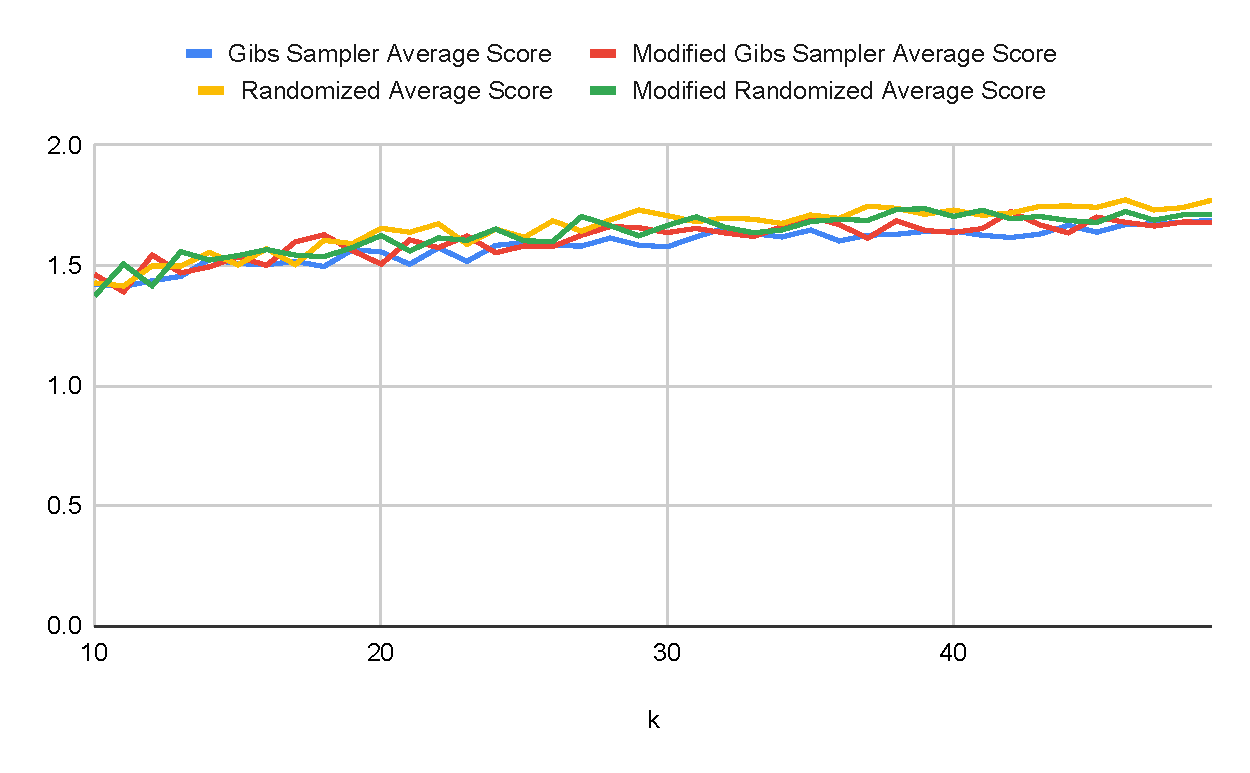
\includegraphics[scale=0.7]{Figs/chart_hm03.pdf}
    \caption{hm03}    
\end{figure}
\begin{figure}[!hptb]
    \centering
    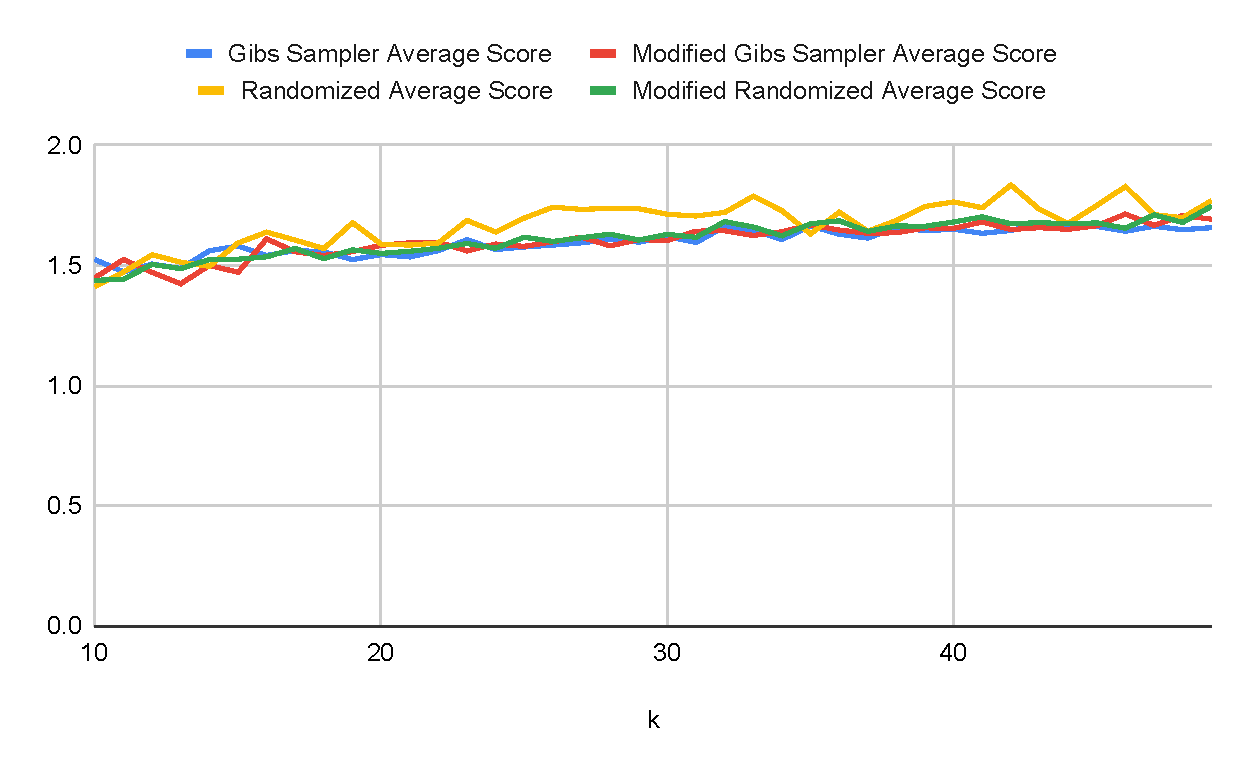
\includegraphics[scale=0.7]{Figs/chart_yst04r.pdf}
    \caption{yst04r}    
\end{figure}
\begin{figure}[!hptb]
    \centering
    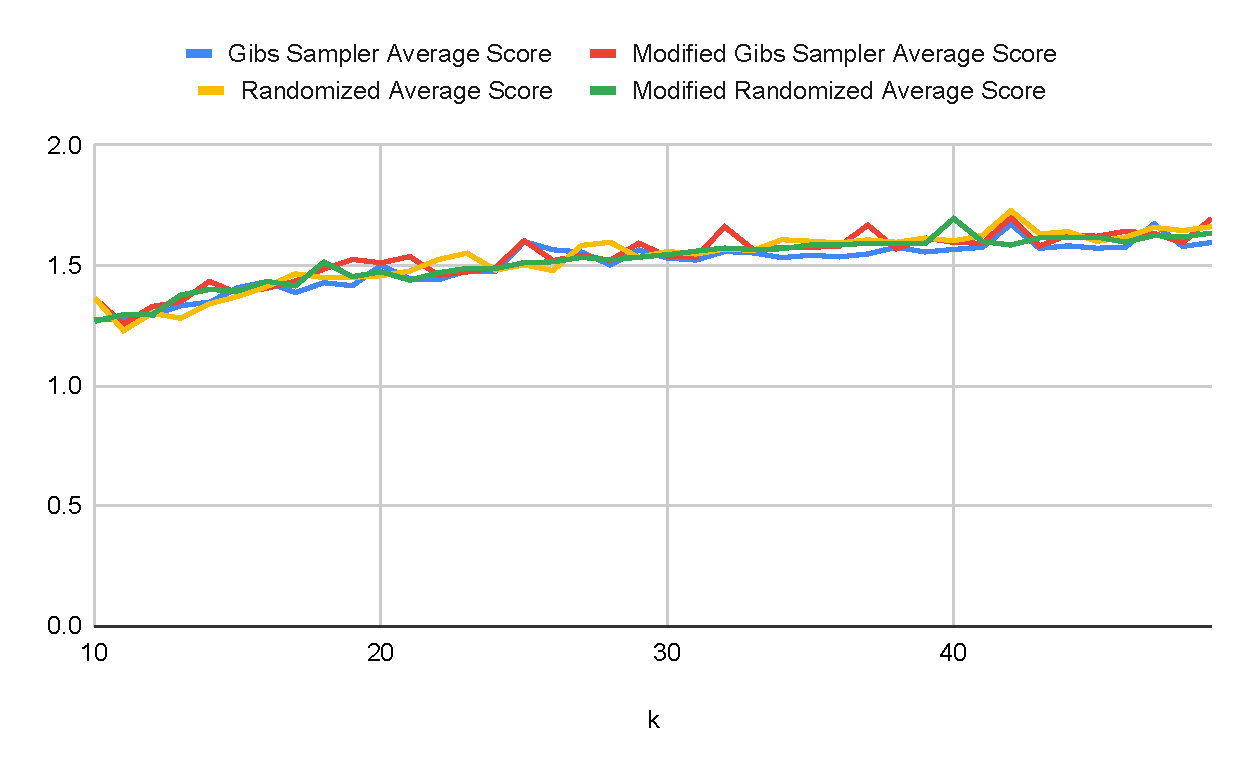
\includegraphics[scale=0.7]{Figs/chart_yst08r.pdf}
    \caption{yst08r}    
\end{figure}
\clearpage
\subsubsection{Comparison of all four methods time vs K values}
For hm03, the results can be found at: \href{https://docs.google.com/spreadsheets/d/1NLuWuYod4BafkorDmi3lj8y2_z9ZDeY42Y-eZODlBIA/edit#gid=350517146}{Supplementary file}\\
For yst04r, the results can be found at: \href{https://docs.google.com/spreadsheets/d/1NLuWuYod4BafkorDmi3lj8y2_z9ZDeY42Y-eZODlBIA/edit#gid=672921087}{Supplementary file}\\
For yst08r, the results can be found at: \href{https://docs.google.com/spreadsheets/d/1NLuWuYod4BafkorDmi3lj8y2_z9ZDeY42Y-eZODlBIA/edit#gid=1580678368}{Supplementary file}
\begin{figure}[!hptb]
    \centering
    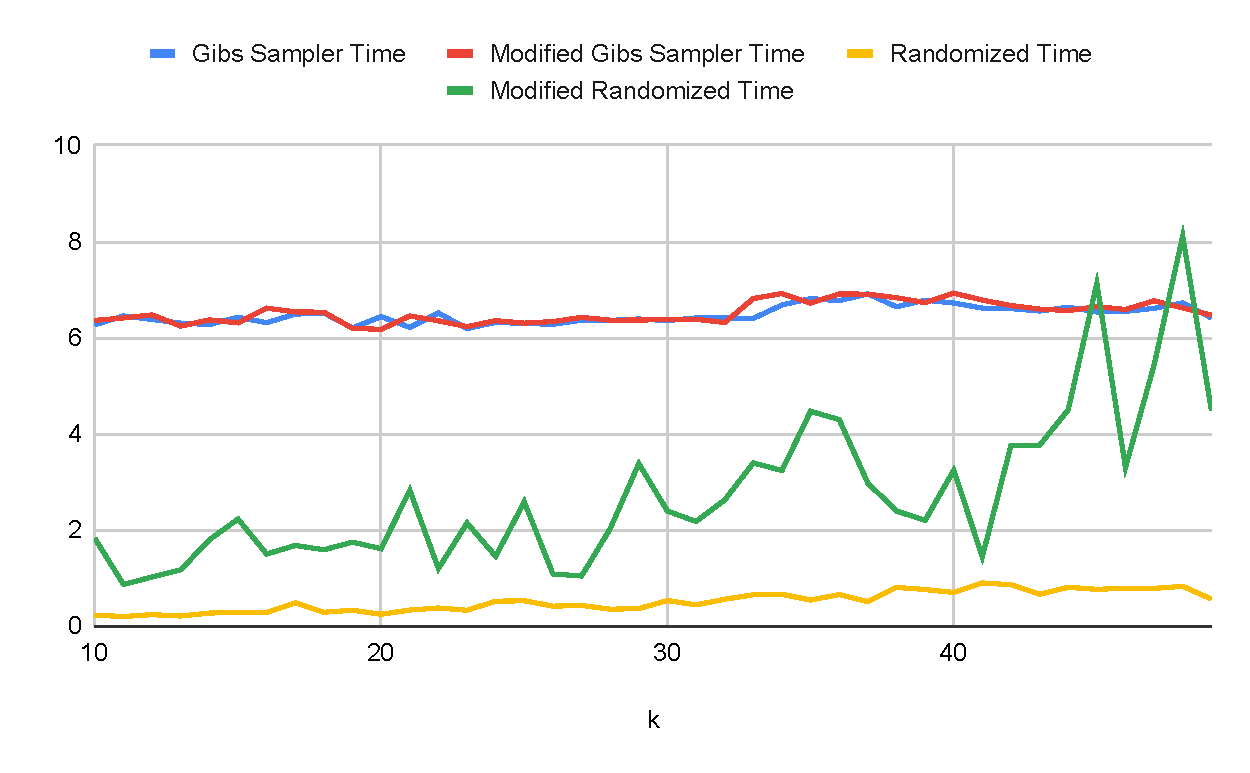
\includegraphics[scale=0.7]{Figs/chart_time_hm03.pdf}
    \caption{hm03}    
\end{figure}
\begin{figure}[!hptb]
    \centering
    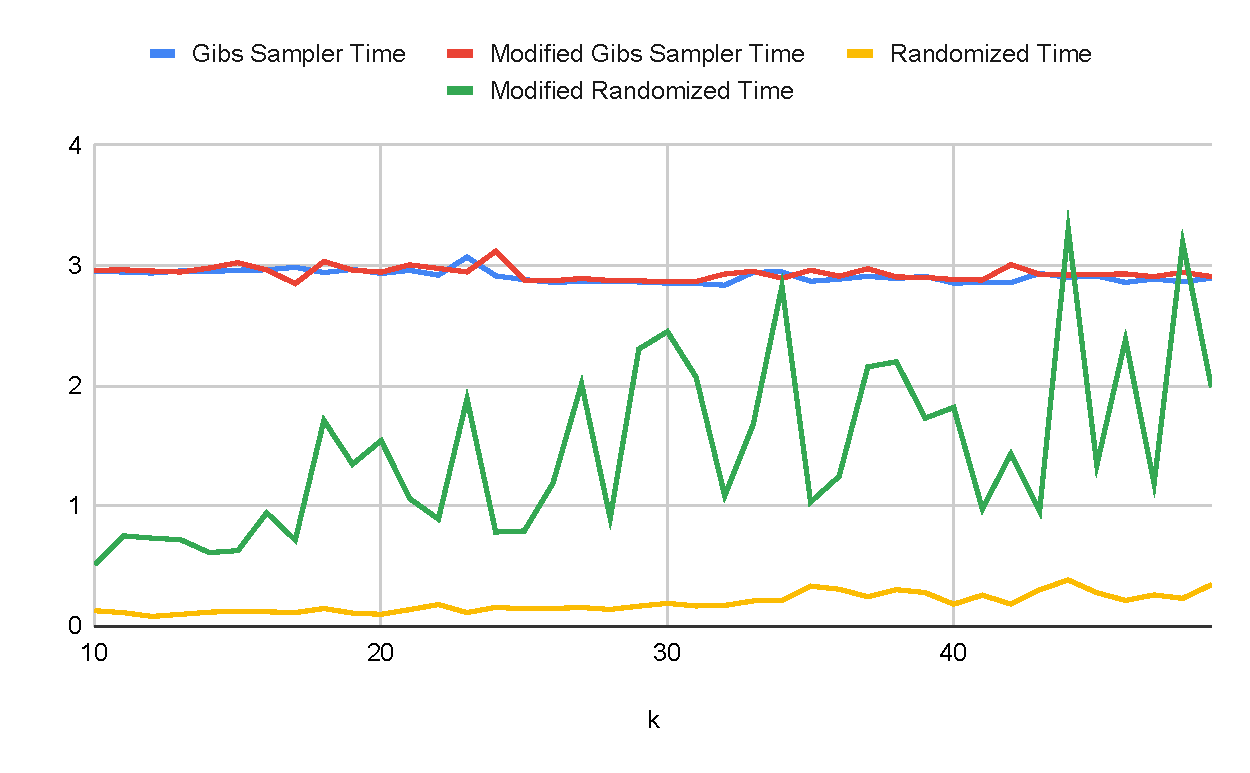
\includegraphics[scale=0.7]{Figs/chart_time_yst04r.pdf}
    \caption{yst04r}    
\end{figure}
\begin{figure}[!hptb]
    \centering
    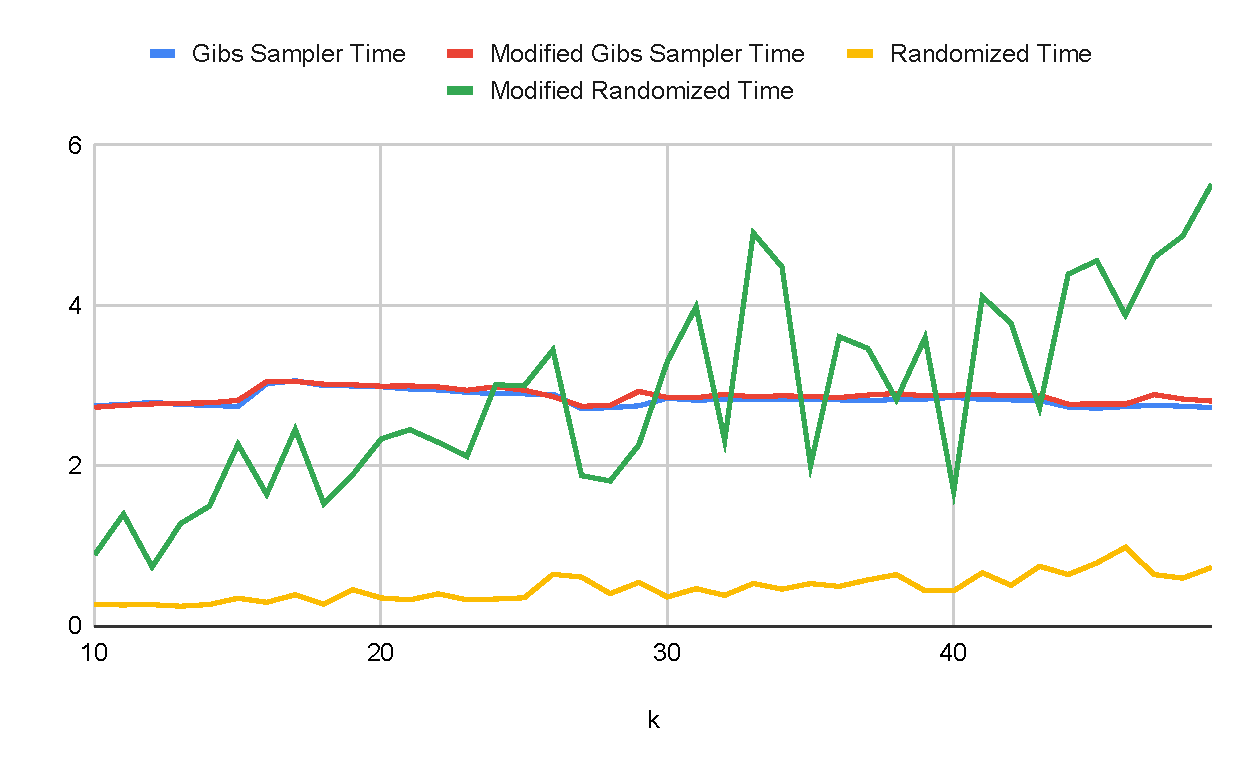
\includegraphics[scale=0.7]{Figs/chart_time_yst08r.pdf}
    \caption{yst08r}    
\end{figure}
\clearpage
\subsubsection{All 8 methods}
Detailed results for first 4 (Randomized Score With Entropy, Randomized Score With Hamming, Modified Randomized Score With Entropy, Modified Randomized Score With Hamming) can be found at:\href{https://docs.google.com/spreadsheets/d/1NLuWuYod4BafkorDmi3lj8y2_z9ZDeY42Y-eZODlBIA/edit#gid=1072118824}{Supplementary file}\\
Detailed results for last 4 (Gibs Sampler Score With Entropy, Gibs Sampler Score With Hamming, Modified Gibs Sampler Score With Entropy, Modified Gibs Sampler Score With Hamming) can be found at:\href{https://docs.google.com/spreadsheets/d/1NLuWuYod4BafkorDmi3lj8y2_z9ZDeY42Y-eZODlBIA/edit#gid=1219346959}{Supplementary file}
\subsubsection{Comparison of all eight methods and MEME}
For all three dataset, we generated results for all 8 methods(Randomized Score With Entropy, Randomized Score With Hamming, Modified Randomized Score With Entropy, Modified Randomized Score With Hamming, Gibs Sampler Score With Entropy, Gibs Sampler Score With Hamming, Modified Gibs Sampler Score With Entropy, Modified Gibs Sampler Score With Hamming) and MEME. Results can be found from: \href{https://docs.google.com/spreadsheets/d/1NLuWuYod4BafkorDmi3lj8y2_z9ZDeY42Y-eZODlBIA/edit#gid=1549331190}{Supplementary file}. It was used for chart generation.\\
From the graph we can see that, MEME performed better for all three dataset.
\begin{figure}[!hptb]
    \centering
    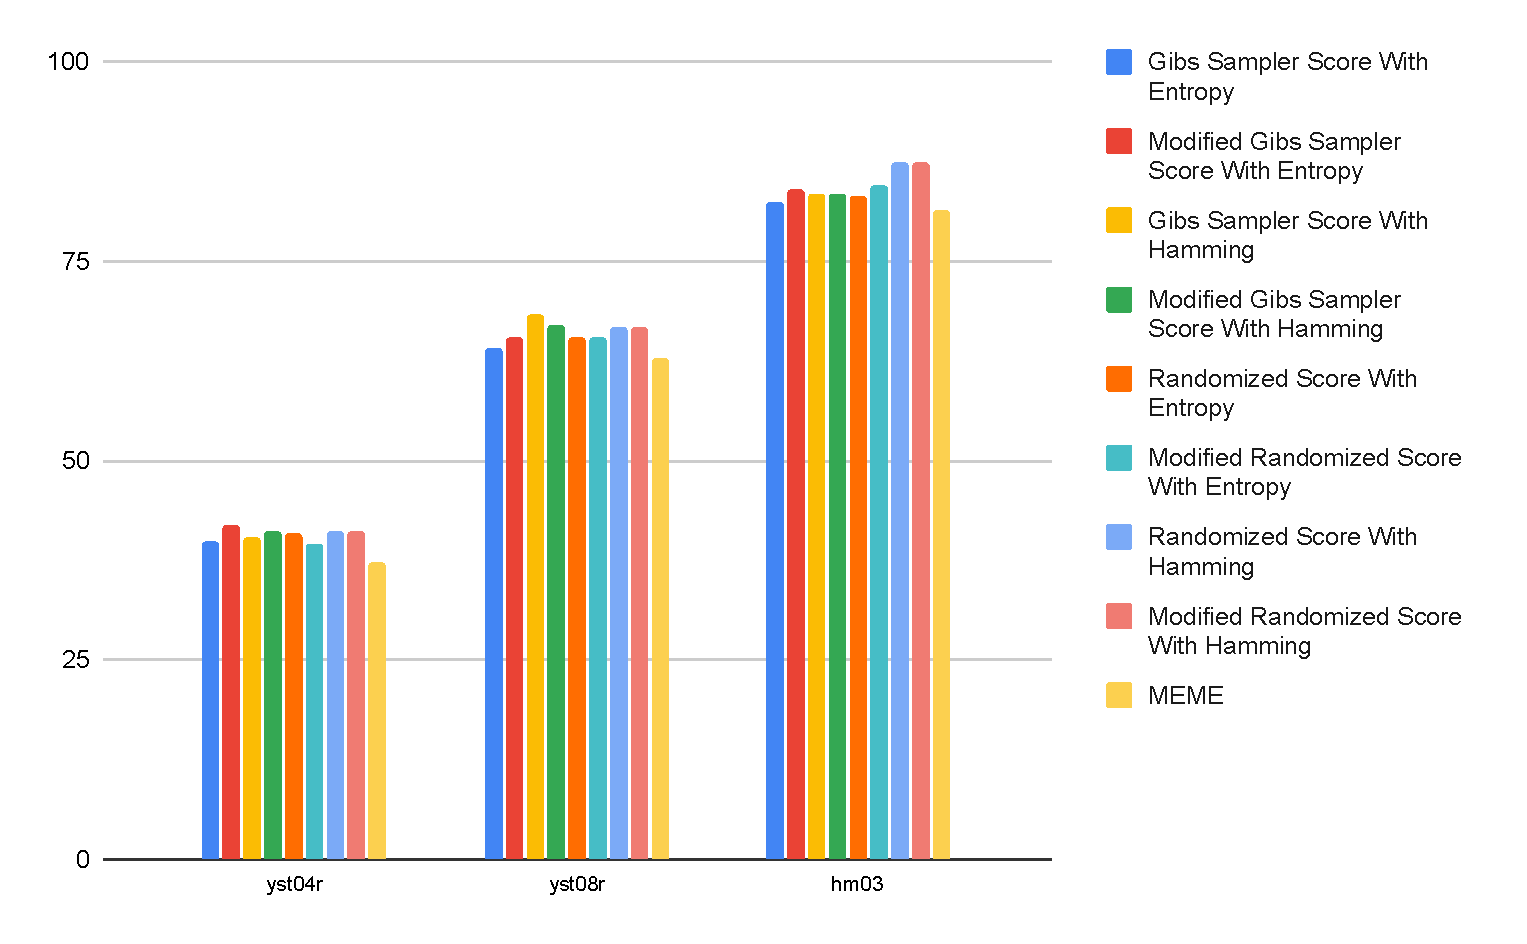
\includegraphics[scale=0.7]{Figs/chart_MEME.pdf}
    \caption{All 8 and MEME}    
\end{figure}
\clearpage
\subsubsection{Comparison of all eight methods and MEME-ChIP}
For all three dataset, we generated results for all 8 methods(Randomized Score With Entropy,Randomized Score With Hamming, Modified Randomized Score With Entropy, Modified Randomized Score With Hamming, Gibs Sampler Score With Entropy, Gibs Sampler Score With Hamming, Modified Gibs Sampler Score With Entropy, Modified Gibs Sampler Score With Hamming) and MEME-ChIP. Results can be found from: \href{https://docs.google.com/spreadsheets/d/1NLuWuYod4BafkorDmi3lj8y2_z9ZDeY42Y-eZODlBIA/edit#gid=1341543901}{Supplementary file}. It was used for chart generation.\\
From the chart, we can see that Modified Randomized
Score With Entropy performed better for yst04r and yst08r. Gibs Sampler Score
With Entropy performed better for hm03.
\begin{figure}[!hptb]
    \centering
    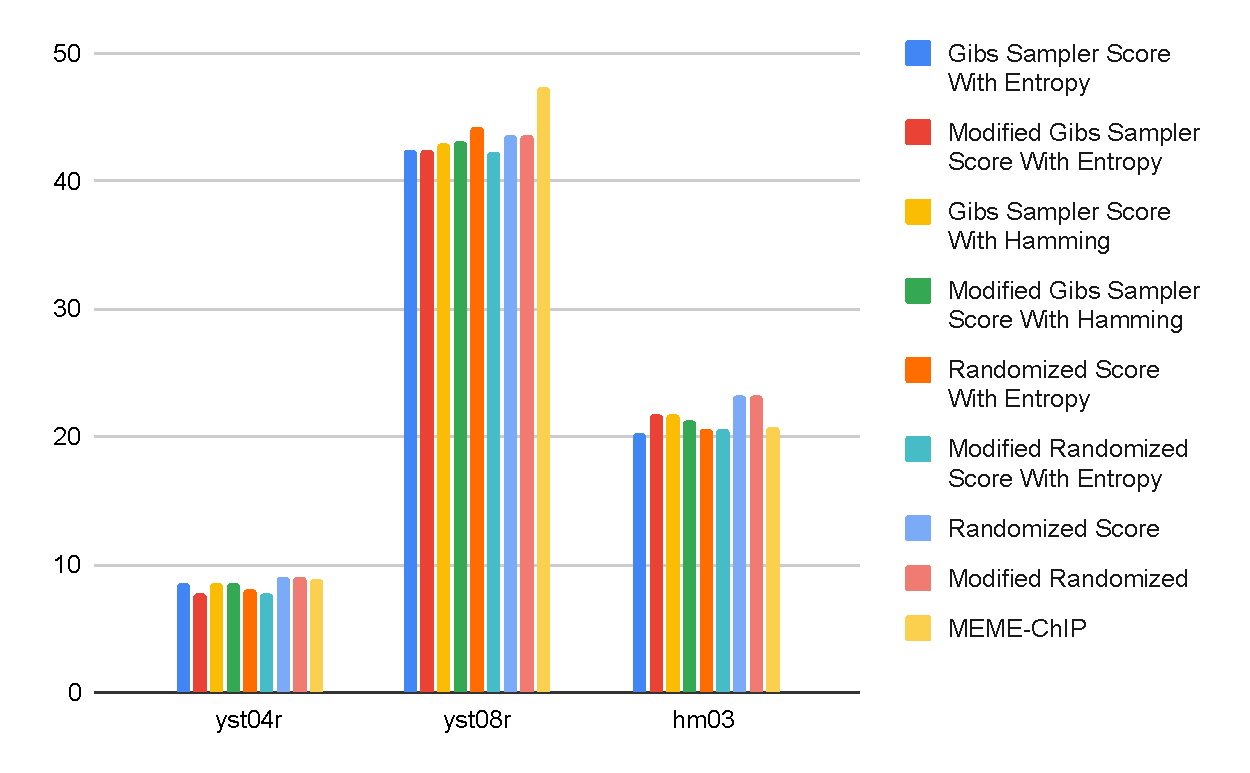
\includegraphics[scale=0.7]{Figs/chart_MEME-ChIP.pdf}
    \caption{All 8 and MEME-ChIP}    
\end{figure}
\clearpage
\subsubsection{MEME vs MEME-ChIP}
We comapred it based on avg entropy motif score. Avg entropy score is calculated using whole entropy divided by k. We can see that MEME perfoms better for yst08r and MEME-ChIP performs better for yst04r and hm03.
\begin{figure}[!hptb]
    \centering
    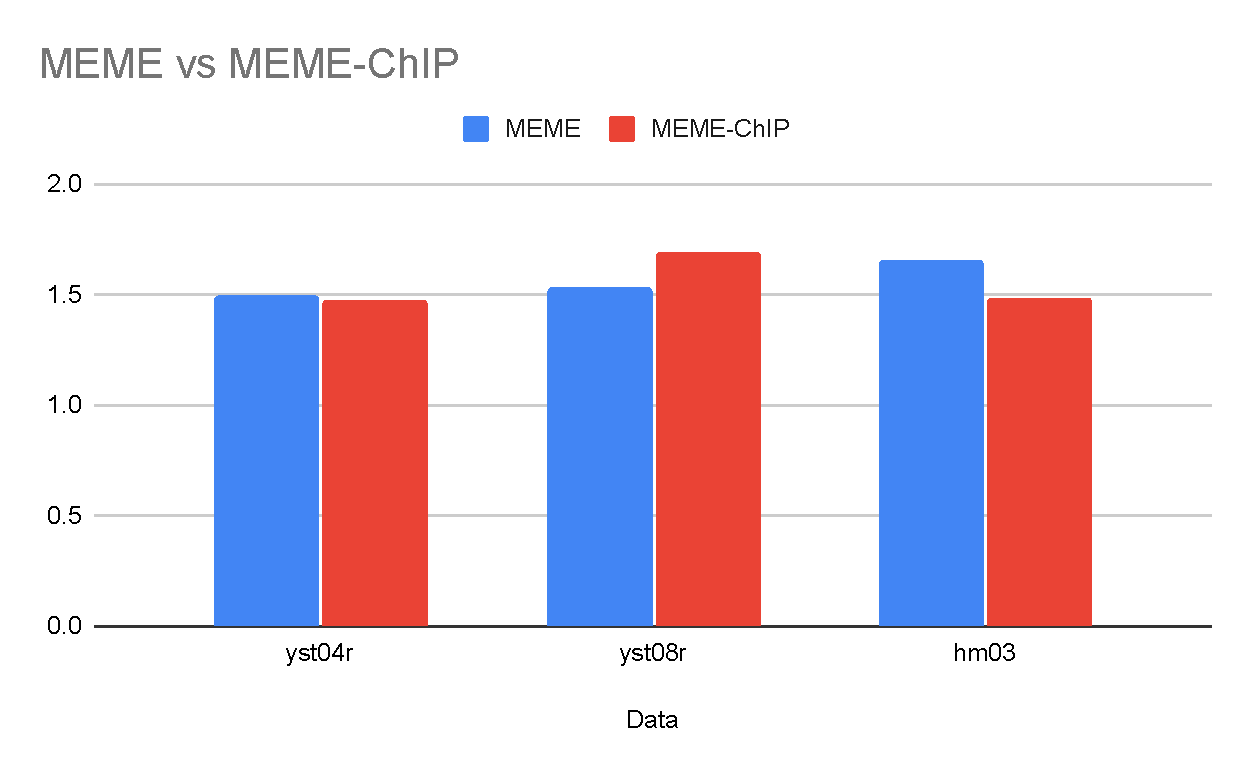
\includegraphics[scale=0.7]{Figs/MEME vs MEME-ChIP.pdf}
    \caption{MEME vs MEME-ChIP}    
\end{figure}
\clearpage
\section{Conclusion}
In the comparison of the main four methods scores with wide range of k values, we can see that Randomized Motif Search perform relatively worse than others for all three dataset and Gibbs Sampler perform well in overall for all three dataset.\\
In the comparison of the main four methods times with wide range of k values, we can see that Randomized Motif Search perform faster than the others. Gibbs Sampler and Modified Gibbs Sampler go with overall constant time. So if we want a faster search, we can go with Randomized Motif Search. If we want a moderate speed search with a constant speed across all k values and better motif, we can go with Gibbs Sampler.\\
In the comparison with all 8 and MEME, MEME performs better. But MEME-ChIP performs worse than the others in all 8 and MEME-ChIP chart. We see, MEME-ChIP perform better than MEME for two dataset in MEME vs MEME-ChIP chart. The contradictions occur due to the less k value of MEME-ChIP. As we have taken avg score entropy values of both MEME and MEME-ChIP motif set and MEME-ChIP has less k value than MEME, MEME-ChIP takes the advantage in the metric. But on the real score evaluations, MEME perform better than MEME-ChIP.
\bibliographystyle{unsrt}
\bibliography{ref}
\end{document}
